\documentclass[11pt,a4paper]{report}
\usepackage[textwidth=37em,vmargin=30mm]{geometry}
\usepackage{calc,xunicode,amsmath,amssymb,paralist,enumitem,tabu,booktabs,datetime2,xeCJK,xeCJKfntef,listings}
\usepackage{tocloft,fancyhdr,tcolorbox,xcolor,graphicx,eso-pic,xltxtra,xelatexemoji}

\newcommand{\envyear}[0]{2024}
\newcommand{\envdatestr}[0]{2024-11-04}
\newcommand{\envfinaldir}[0]{webdb/2024/20241104/final}

\usepackage[hidelinks]{hyperref}
\hypersetup{
    colorlinks=false,
    pdfpagemode=FullScreen,
    pdftitle={Web Digest - \envdatestr}
}

\setlength{\cftbeforechapskip}{10pt}
\renewcommand{\cftchapfont}{\rmfamily\bfseries\large\raggedright}
\setlength{\cftbeforesecskip}{2pt}
\renewcommand{\cftsecfont}{\sffamily\small\raggedright}

\setdefaultleftmargin{2em}{2em}{1em}{1em}{1em}{1em}

\usepackage{xeCJK,xeCJKfntef}
\xeCJKsetup{PunctStyle=plain,RubberPunctSkip=false,CJKglue=\strut\hskip 0pt plus 0.1em minus 0.05em,CJKecglue=\strut\hskip 0.22em plus 0.2em}
\XeTeXlinebreaklocale "zh"
\XeTeXlinebreakskip = 0pt


\setmainfont{Brygada 1918}
\setromanfont{Brygada 1918}
\setsansfont{IBM Plex Sans}
\setmonofont{JetBrains Mono NL}
\setCJKmainfont{Noto Serif CJK SC}
\setCJKromanfont{Noto Serif CJK SC}
\setCJKsansfont{Noto Sans CJK SC}
\setCJKmonofont{Noto Sans CJK SC}

\setlength{\parindent}{0pt}
\setlength{\parskip}{8pt}
\linespread{1.15}

\lstset{
	basicstyle=\ttfamily\footnotesize,
	numbersep=5pt,
	backgroundcolor=\color{black!5},
	showspaces=false,
	showstringspaces=false,
	showtabs=false,
	tabsize=2,
	captionpos=b,
	breaklines=true,
	breakatwhitespace=true,
	breakautoindent=true,
	linewidth=\textwidth
}






\newcommand{\coverpic}[2]{
    % argv: itemurl, authorname
    Cover photo by #2~~(\href{#1}{#1})
}
\newcommand{\makeheader}[0]{
    \begin{titlepage}
        % \newgeometry{hmargin=15mm,tmargin=21mm,bmargin=12mm}
        \begin{center}
            
            \rmfamily\scshape
            \fontspec{BaskervilleF}
            \fontspec{Old Standard}
            \fontsize{59pt}{70pt}\selectfont
            WEB\hfill DIGEST
            
            \vfill
            % \vskip 30pt
            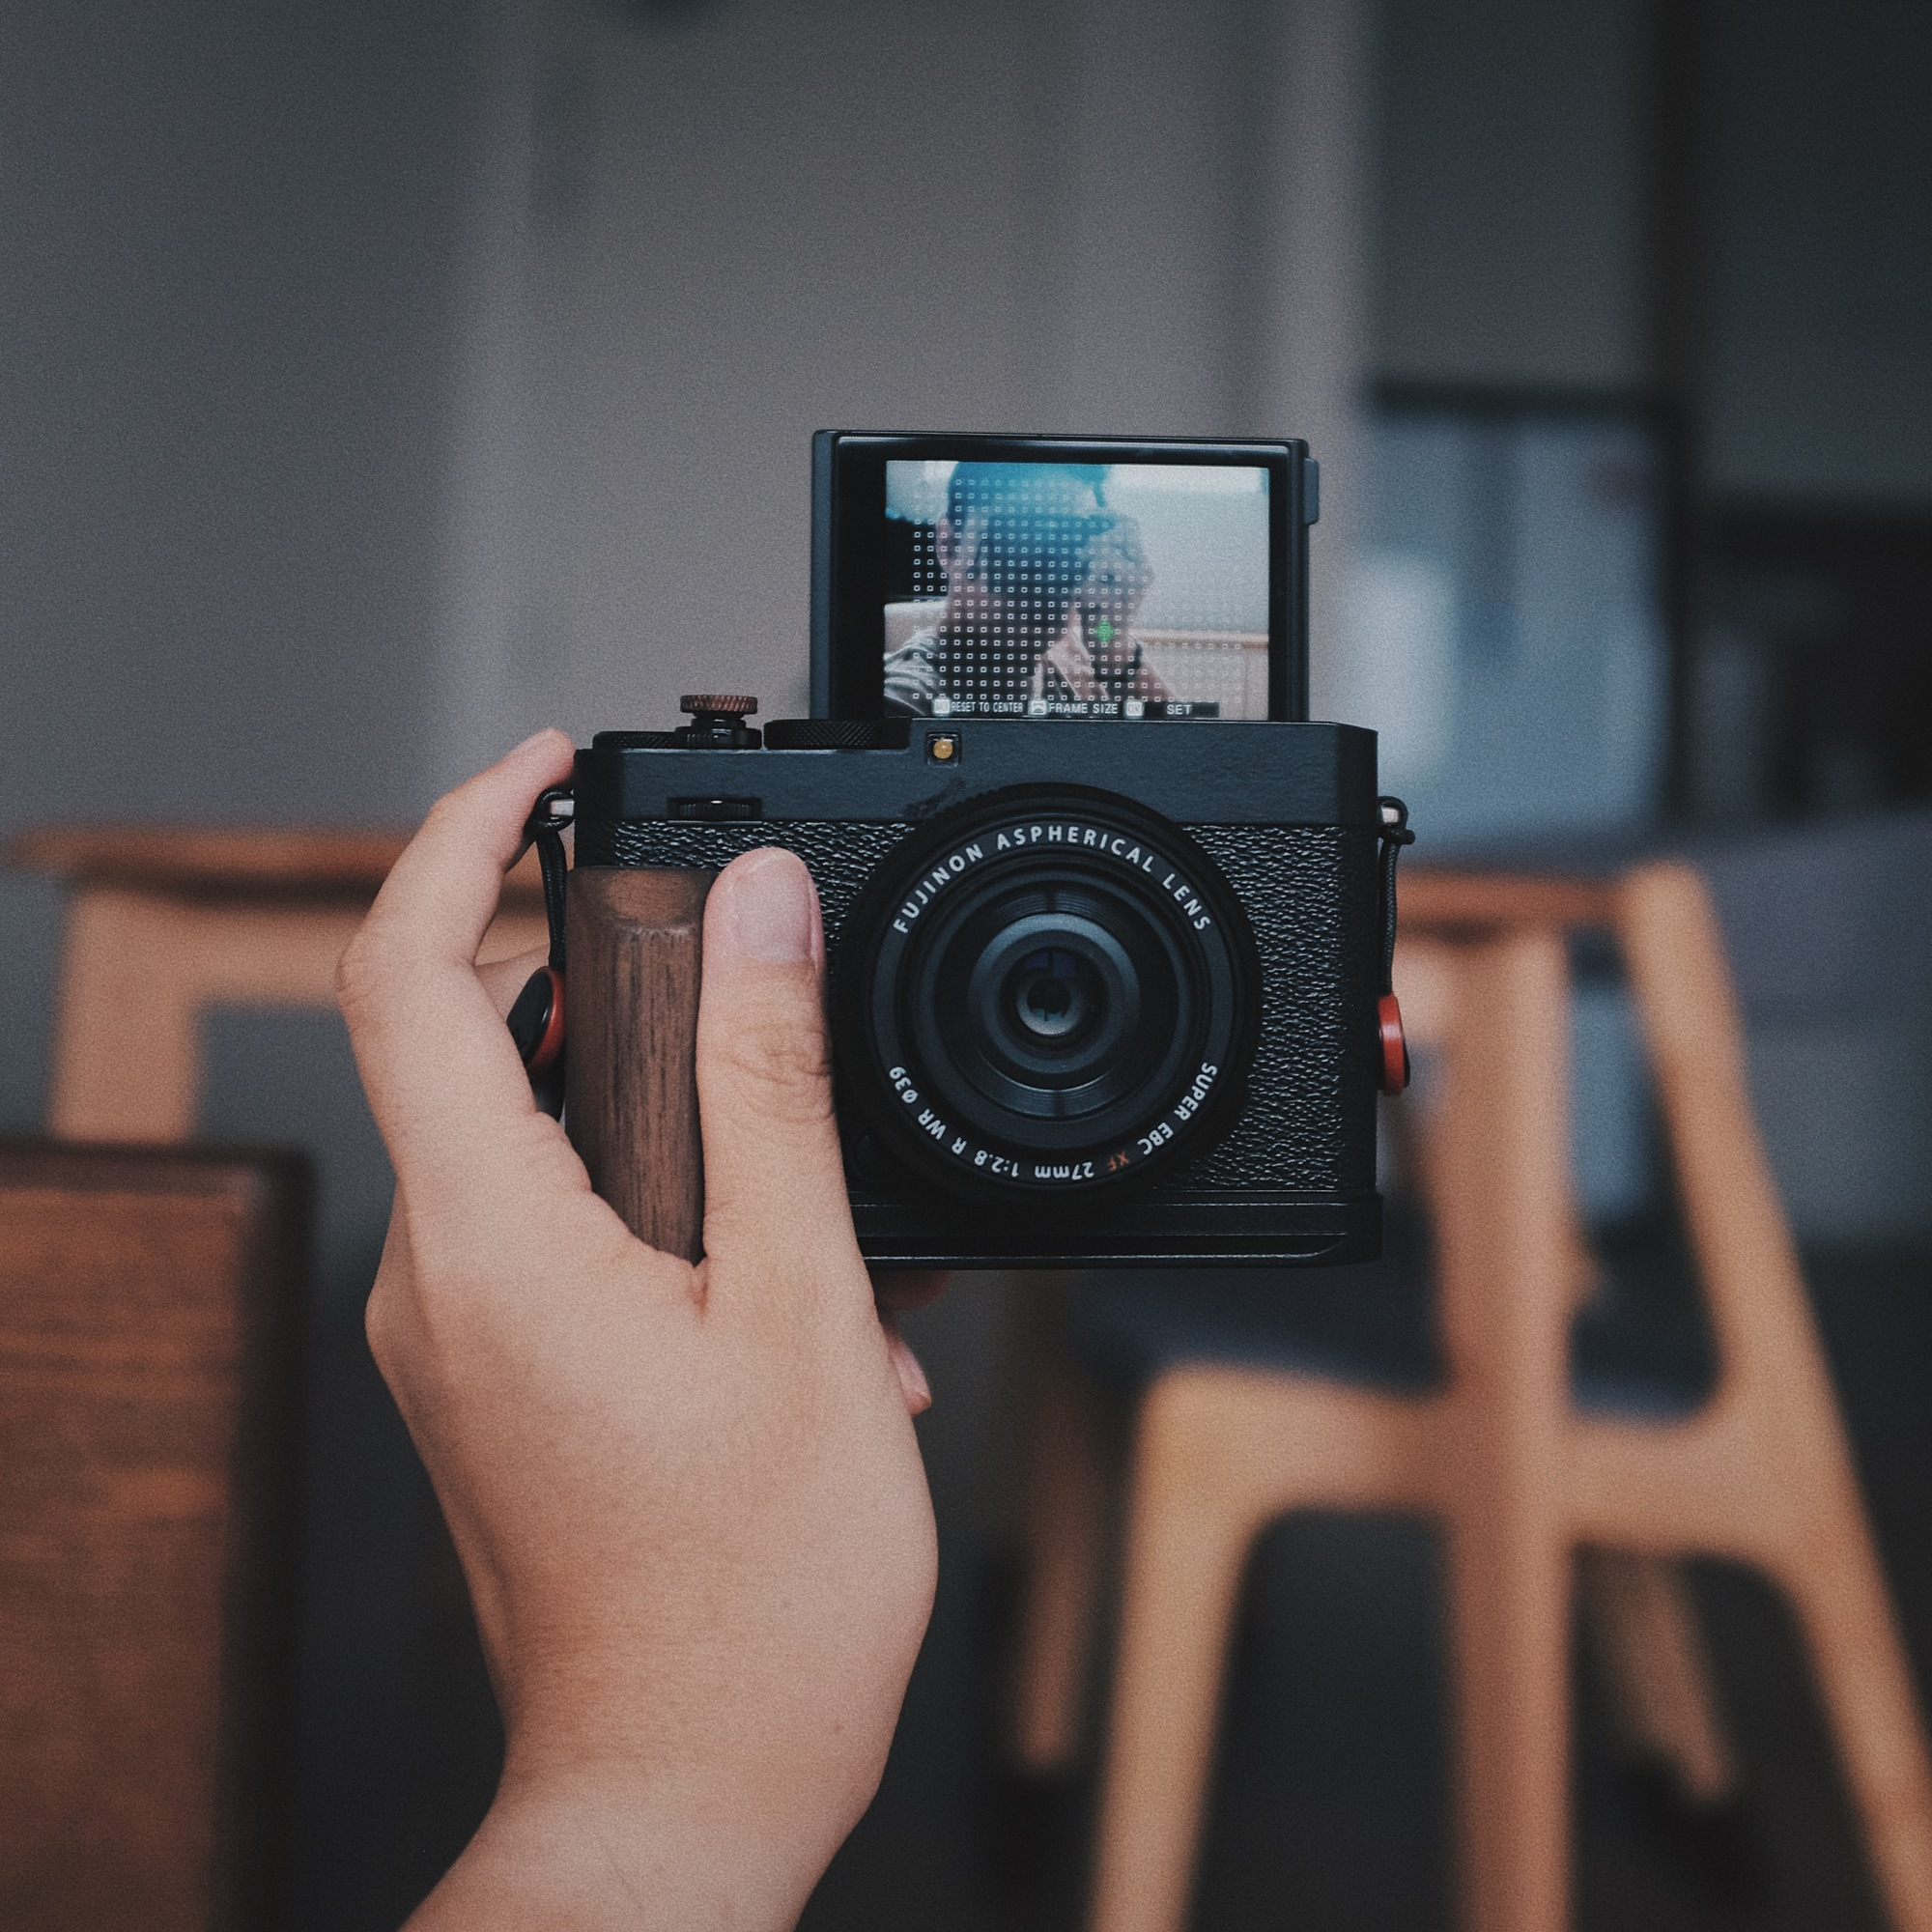
\includegraphics[width=\linewidth]{\envfinaldir/coverpic-prod.jpg}\par
            % \vskip 30pt
            \vfill

            \normalsize\rmfamily\scshape
            \copyright{} The Web Digest Project \hfill\large \envdatestr
        \end{center}
    \end{titlepage}
    % \restoregeometry
}
\newcommand{\simplehref}[1]{%
    \textcolor{blue!80!green}{\href{#1}{#1}}%
}
\renewcommand{\contentsname}{\center\Huge\sffamily\bfseries Contents\par\vskip 20pt}
\newcounter{ipartcounter}
\setcounter{ipartcounter}{0}
\newcommand{\ipart}[1]{
    % \vskip 20pt
    \clearpage
    \stepcounter{ipartcounter}
    \phantomsection
    \addcontentsline{toc}{chapter}{#1}
    % \begin{center}
    %     \Huge
    %     \sffamily\bfseries
    %     #1
    % \end{center}
    % \vskip 20pt plus 7pt
}
\newcounter{ichaptercounter}
\setcounter{ichaptercounter}{0}
\newcommand{\ichapter}[1]{
    % \vskip 20pt
    \clearpage
    \stepcounter{ichaptercounter}
    \phantomsection
    \addcontentsline{toc}{section}{\numberline{\arabic{ichaptercounter}}#1}
    \begin{center}
        \Huge
        \sffamily\bfseries
        #1
    \end{center}
    \vskip 20pt plus 7pt
}
\newcommand{\entrytitlefont}[1]{\subsection*{\raggedright\Large\sffamily\bfseries#1}}
\newcommand{\entryitemGeneric}[2]{
    % argv: title, url
    \parbox{\linewidth}{
        \entrytitlefont{#1}\par\vskip 5pt
        \footnotesize\ttfamily\mdseries
        \simplehref{#2}
    }\vskip 11pt plus 11pt minus 1pt
}
\newcommand{\entryitemGithub}[3]{
    % argv: title, url, desc
    \parbox{\linewidth}{
        \entrytitlefont{#1}\par\vskip 5pt
        \footnotesize\ttfamily\mdseries
        \simplehref{#2}\par\vskip 5pt
        \small\rmfamily\mdseries#3
    }\vskip 11pt plus 11pt minus 1pt
}
\newcommand{\entryitemAp}[3]{
    % argv: title, url, desc
    \parbox{\linewidth}{
        \entrytitlefont{#1}\par\vskip 5pt
        \footnotesize\ttfamily\mdseries
        \simplehref{#2}\par\vskip 5pt
        \small\rmfamily\mdseries#3
    }\vskip 11pt plus 11pt minus 1pt
}
\newcommand{\entryitemHackernews}[3]{
    % argv: title, hnurl, rawurl
    % \parbox{\linewidth}{
    %     \entrytitlefont{#1}\par\vskip 5pt
    %     \footnotesize\ttfamily\mdseries
    %     \simplehref{#3}\par
    %     \textcolor{black!50}{\href{#2}{#2}}
    % }\vskip 11pt plus 11pt minus 1pt
    \begin{minipage}{\linewidth}
            \entrytitlefont{#1}\par\vskip 5pt
            \footnotesize\ttfamily\mdseries
            \simplehref{#3}\par
            \textcolor{black!50}{\href{#2}{#2}}
    \end{minipage}\par\vskip 11pt plus 11pt minus 1pt
}







\begin{document}

\makeheader

\tableofcontents\clearpage




\ipart{Developers}
\ichapter{Hacker News}
\entryitemTwoLinks{Project Sid: Many-agent simulations toward AI civilization}{https://news.ycombinator.com/item?id=42035319}{https://github.com/altera-al/project-sid}

\entryitemTwoLinks{pg\_flo – Stream, transform, and re-route PostgreSQL data in real-time}{https://news.ycombinator.com/item?id=42034237}{https://www.pgflo.io/}

\entryitemTwoLinks{Auth Wiki}{https://news.ycombinator.com/item?id=42033295}{https://auth.wiki/}

\entryitemTwoLinks{Touchscreens are out, and tactile controls are back}{https://news.ycombinator.com/item?id=42033241}{https://spectrum.ieee.org/touchscreens}

\entryitemTwoLinks{If you need the money, don't take the job}{https://news.ycombinator.com/item?id=42032638}{https://bitfieldconsulting.com/posts/need-money}

\entryitemTwoLinks{Matrix 2.0 Is Here}{https://news.ycombinator.com/item?id=42032387}{https://matrix.org/blog/2024/10/29/matrix-2.0-is-here/?resubmit}

\entryitemTwoLinks{Speed, scale and reliability: 25 years of Google datacenter networking evolution}{https://news.ycombinator.com/item?id=42031169}{https://cloud.google.com/blog/products/networking/speed-scale-reliability-25-years-of-data-center-networking}

\entryitemTwoLinks{Ask HN: What would you preserve if the internet were to go down tomorrow?}{https://news.ycombinator.com/item?id=42030832}{https://news.ycombinator.com/item?id=42030832}

\entryitemTwoLinks{Ractor – a Rust Actor Framework}{https://news.ycombinator.com/item?id=42030625}{https://slawlor.github.io/ractor/quickstart/}

\entryitemTwoLinks{Security flaws found in Nvidia GeForce GPUs}{https://news.ycombinator.com/item?id=42030463}{https://www.pcworld.com/article/2504035/security-flaws-found-in-all-nvidia-geforce-gpus-update-drivers-asap.html}

\entryitemTwoLinks{Spann: Highly-Efficient Billion-Scale Approximate Nearest Neighbor Search (2021)}{https://news.ycombinator.com/item?id=42028873}{https://arxiv.org/abs/2111.08566}

\entryitemTwoLinks{Next Generation Out of Band Garbage Collection}{https://news.ycombinator.com/item?id=42028833}{https://railsatscale.com/2024-10-23-next-generation-oob-gc/}

\entryitemTwoLinks{Eighty Years of the Finite Element Method (2022)}{https://news.ycombinator.com/item?id=42028569}{https://link.springer.com/article/10.1007/s11831-022-09740-9}

\entryitemTwoLinks{Show HN: A minimalist (brutalist?) website for sharing all your links}{https://news.ycombinator.com/item?id=42027654}{https://lynx.boo}

\entryitemTwoLinks{Britain's postwar sugar craze confirms harms of sweet diets in early life}{https://news.ycombinator.com/item?id=42027564}{https://www.science.org/content/article/britain-s-postwar-sugar-craze-confirms-harms-sweet-diets-early-life}

\entryitemTwoLinks{Show HN: Someday, Open-Source Calendly Alternative for Gmail / Google App Script}{https://news.ycombinator.com/item?id=42027187}{https://github.com/rbbydotdev/someday}

\entryitemTwoLinks{Cash: A small jQuery alternative for modern browsers}{https://news.ycombinator.com/item?id=42026054}{https://github.com/fabiospampinato/cash}

\entryitemTwoLinks{SpawELO – small free matchmaking system for LAN parties}{https://news.ycombinator.com/item?id=42025469}{https://blog.spawek.com/SpawELO}

\entryitemTwoLinks{Weird Lexical Syntax}{https://news.ycombinator.com/item?id=42024727}{https://justine.lol/lex/}

\entryitemTwoLinks{SmolLM2}{https://news.ycombinator.com/item?id=42024661}{https://simonwillison.net/2024/Nov/2/smollm2/}\ichapter{Phoronix}
\entryitemGeneric{\hskip 0pt{}Rust-Based Redox OS Gets RISC-V Working, Also Now Booting On The Raspberry Pi 4}{https://www.phoronix.com/news/Redox-OS-For-October-2024}

\entryitemGeneric{\hskip 0pt{}AMD Heterogeneous CPU Design Topology Patches Coming For Linux 6.13}{https://www.phoronix.com/news/AMD-Hetero-Topo-Linux-6.13}

\entryitemGeneric{\hskip 0pt{}Linux Mint Working On Night Light For Cinnamon, Collaborating With Framework Computer}{https://www.phoronix.com/news/Linux-Mint-Framework-Collab}

\entryitemGeneric{\hskip 0pt{}Nice Performance Gains With SVT-AV1 2.3 Encoding On The System76 Thelio Astra}{https://www.phoronix.com/news/SVT-AV1-2.3-ARM-Performance}

\entryitemGeneric{\hskip 0pt{}Apple Silicon OpenGL/Vulkan Drivers Updated This Week For Mesa 24.3}{https://www.phoronix.com/news/Apple-GL-VLK-Mesa-24.3-Okt-Sync}

\entryitemGeneric{\hskip 0pt{}Snapdragon X1 Elite CPUFreq Support Revised In Latest Linux Patches}{https://www.phoronix.com/news/Snapdragon-X1-Elite-CPUFreq-V7}

\entryitemGeneric{\hskip 0pt{}FreeBSD 14.2 Beta 1 Released To Work Toward This Next Release}{https://www.phoronix.com/news/FreeBSD-14.2-Beta-1-Released}

\entryitemGeneric{\hskip 0pt{}Cloudflare's Pingora 0.4 Rust Framework Released With Experimental Windows Support}{https://www.phoronix.com/news/Cloudflare-Pingora-0.4}

\entryitemGeneric{\hskip 0pt{}Genode-Based Sculpt OS 24.10 Introduces Multi-Monitor Support}{https://www.phoronix.com/news/Genode-Sculpt-OS-24.10}\ichapter{Dribbble}
\entryitemGeneric{\hskip 0pt{}Lootbox}{https://dribbble.com/shots/24875582}

\entryitemGeneric{\hskip 0pt{}Internal Universe 🪐✨}{https://dribbble.com/shots/24870294}

\entryitemGeneric{\hskip 0pt{}Gulfstream x theory11 Playing Cards}{https://dribbble.com/shots/24869176}

\entryitemGeneric{\hskip 0pt{}Negative yet Positive Vol.7}{https://dribbble.com/shots/24868890}

\entryitemGeneric{\hskip 0pt{}Onton - Responsive Logo Design}{https://dribbble.com/shots/24866015}

\entryitemGeneric{\hskip 0pt{}Solufacil}{https://dribbble.com/shots/24869750}

\entryitemGeneric{\hskip 0pt{}Raw E}{https://dribbble.com/shots/24869489}

\entryitemGeneric{\hskip 0pt{}Ampersand 3D Logo}{https://dribbble.com/shots/24869500}

\entryitemGeneric{\hskip 0pt{}Rooster}{https://dribbble.com/shots/24854380}

\entryitemGeneric{\hskip 0pt{}cipher}{https://dribbble.com/shots/24855823}

\entryitemGeneric{\hskip 0pt{}"Amphiprion Ocellaris" - Daily art, NFT art}{https://dribbble.com/shots/24854577}

\entryitemGeneric{\hskip 0pt{}Bento Cards v.4 – E-Commerce}{https://dribbble.com/shots/24849627}

\entryitemGeneric{\hskip 0pt{}Neobanking Mobile App Interactions}{https://dribbble.com/shots/24848696}

\entryitemGeneric{\hskip 0pt{}FC Shakhtar Donetsk App. The Concept. Part 2}{https://dribbble.com/shots/24848383}

\entryitemGeneric{\hskip 0pt{}xflow Logo Design - X, Waves}{https://dribbble.com/shots/24847689}

\entryitemGeneric{\hskip 0pt{}The Future has landed ✈️}{https://dribbble.com/shots/24848230}

\entryitemGeneric{\hskip 0pt{}Converse Logo Redesign Concept}{https://dribbble.com/shots/24850036}

\entryitemGeneric{\hskip 0pt{}F Logo}{https://dribbble.com/shots/24850079}

\entryitemGeneric{\hskip 0pt{}ML Fashion 10/10}{https://dribbble.com/shots/24851262}

\entryitemGeneric{\hskip 0pt{}Amplemarket Logo Design}{https://dribbble.com/shots/24843224}

\entryitemGeneric{\hskip 0pt{}Streaming Data}{https://dribbble.com/shots/24838862}

\entryitemGeneric{\hskip 0pt{}It's not a feature, it's a bug}{https://dribbble.com/shots/24844082}

\entryitemGeneric{\hskip 0pt{}Cute Raccoon}{https://dribbble.com/shots/24843120}

\entryitemGeneric{\hskip 0pt{}Nero Code UI concept}{https://dribbble.com/shots/24843816}


\ipart{Developers~~~~(zh-Hans)}
\ichapter{Solidot}
\entryitemGeneric{\hskip 0pt{}Steam 平台 Linux 份额突破 2\%}{https://www.solidot.org/story?sid=79667}

\entryitemGeneric{\hskip 0pt{}前三季度全国结婚登记人数减少逾 90 万对}{https://www.solidot.org/story?sid=79666}

\entryitemGeneric{\hskip 0pt{}第四名 FTX 高管被判没收 110 亿美元}{https://www.solidot.org/story?sid=79665}

\entryitemGeneric{\hskip 0pt{}苹果收购图像编辑应用 Pixelmator}{https://www.solidot.org/story?sid=79664}

\entryitemGeneric{\hskip 0pt{}日本东京高院裁定不承认同性婚姻违宪}{https://www.solidot.org/story?sid=79663}

\entryitemGeneric{\hskip 0pt{}英伟达取代英特尔进入道琼斯工业平均指数}{https://www.solidot.org/story?sid=79662}

\entryitemGeneric{\hskip 0pt{}Linus Torvalds 用电动汽车取代了燃油汽车}{https://www.solidot.org/story?sid=79661}

\entryitemGeneric{\hskip 0pt{}随着减肥药的流行减肥手术减少了四分之一}{https://www.solidot.org/story?sid=79660}

\entryitemGeneric{\hskip 0pt{}蝙蝠仅靠回声可导航数公里}{https://www.solidot.org/story?sid=79659}

\entryitemGeneric{\hskip 0pt{}研究发现猴子永远也写不出莎士比亚著作}{https://www.solidot.org/story?sid=79658}

\entryitemGeneric{\hskip 0pt{}科技行业盛行发布``虚假招聘''}{https://www.solidot.org/story?sid=79657}

\entryitemGeneric{\hskip 0pt{}生命早期限糖可预防成年后罹患糖尿病和高血压}{https://www.solidot.org/story?sid=79656}

\entryitemGeneric{\hskip 0pt{}日本限制边骑车边打手机}{https://www.solidot.org/story?sid=79655}

\entryitemGeneric{\hskip 0pt{}栉水母能逆转衰老}{https://www.solidot.org/story?sid=79654}

\entryitemGeneric{\hskip 0pt{}微软向 Windows 10 用户提供一次性 30 美元的一年安全更新}{https://www.solidot.org/story?sid=79653}

\entryitemGeneric{\hskip 0pt{}Android 16 将于 2025 年二季度发布}{https://www.solidot.org/story?sid=79652}

\entryitemGeneric{\hskip 0pt{}微软再次推迟 Windows Recall}{https://www.solidot.org/story?sid=79651}\ichapter{V2EX}
\entryitemGeneric{\hskip 0pt{}[Apple] 买了苹果新 magic trackpad,发现真的是太蠢了,大家要注意这个坑}{https://www.v2ex.com/t/1086290}

\entryitemGeneric{\hskip 0pt{}[前端开发] 在 iPhone safari 选择添加到书签后,书签里不显示网站的图标,怎么破?}{https://www.v2ex.com/t/1086289}

\entryitemGeneric{\hskip 0pt{}[问与答] ✳️这个符号的软件是什么,还请大神帮我解答一下。}{https://www.v2ex.com/t/1086287}

\entryitemGeneric{\hskip 0pt{}[程序员] 2024 年,选择 Cloudflare Pages 还是 Vercel 部署好?}{https://www.v2ex.com/t/1086286}

\entryitemGeneric{\hskip 0pt{}[Apple] 完蛋.. 京东的 mac mini 国补数量满了.. 现在购买已经没补贴了..}{https://www.v2ex.com/t/1086285}

\entryitemGeneric{\hskip 0pt{}[Apple] 24 寸 4k 显示器怎么选?}{https://www.v2ex.com/t/1086280}

\entryitemGeneric{\hskip 0pt{}[程序员] 一个 webview Python 绑定,欢迎试用}{https://www.v2ex.com/t/1086279}

\entryitemGeneric{\hskip 0pt{}[NAS] 硬件还是软件 RAID?}{https://www.v2ex.com/t/1086278}

\entryitemGeneric{\hskip 0pt{}[分享创造] 我梦见和英伟达创始人黄仁勋一起吃饭散步,意味着什么?}{https://www.v2ex.com/t/1086273}

\entryitemGeneric{\hskip 0pt{}[宽带症候群] 用 singbox 代理,模式到底选 Tproxy 还是 Tun?}{https://www.v2ex.com/t/1086272}

\entryitemGeneric{\hskip 0pt{}[git] 推荐一下自己一直在维护的 gcop: git ai copilot,自动化撰写优质的 git commit message、加速 git workflow}{https://www.v2ex.com/t/1086271}

\entryitemGeneric{\hskip 0pt{}[云修电脑] 有没有 PC 硬件专家,问个 PC 无法启动的问题}{https://www.v2ex.com/t/1086270}

\entryitemGeneric{\hskip 0pt{}[程序员] 拆机小白问一下几个小问题?}{https://www.v2ex.com/t/1086269}

\entryitemGeneric{\hskip 0pt{}[分享创造] 不会写代码的我用 cursor 六小时,写了一个文章摘要的小工具}{https://www.v2ex.com/t/1086268}

\entryitemGeneric{\hskip 0pt{}[问与答] 家里用小米指纹锁的麻烦进来下}{https://www.v2ex.com/t/1086267}

\entryitemGeneric{\hskip 0pt{}[Apple] 打算买美版全新 16pm 大修机,求打醒,都大修了,要不要顺便扩容 1t}{https://www.v2ex.com/t/1086266}

\entryitemGeneric{\hskip 0pt{}[Linux] 有人买到了 Hackberry Linux 便携终端吗?}{https://www.v2ex.com/t/1086264}

\entryitemGeneric{\hskip 0pt{}[成都] 工业风扇,除甲醛,线下自提}{https://www.v2ex.com/t/1086263}

\entryitemGeneric{\hskip 0pt{}[职场话题] 全栈工程师现在多吗}{https://www.v2ex.com/t/1086261}

\entryitemGeneric{\hskip 0pt{}[OpenWrt] 用 immoralwrt 安装网络代理客户端 passwall2}{https://www.v2ex.com/t/1086260}

\entryitemGeneric{\hskip 0pt{}[VPS] [性价比最高的 vps] 季付 2.8 刀/月 [联通快乐鸡]}{https://www.v2ex.com/t/1086259}

\entryitemGeneric{\hskip 0pt{}[分享发现] 只要三千一还能用 apple intelligence 的 iPad mini7 还是很香!}{https://www.v2ex.com/t/1086258}

\entryitemGeneric{\hskip 0pt{}[Windows] 拯救者清完灰自动重启}{https://www.v2ex.com/t/1086256}

\entryitemGeneric{\hskip 0pt{}[问与答] finalshell 问题}{https://www.v2ex.com/t/1086255}

\entryitemGeneric{\hskip 0pt{}[酷工作] 兄弟们,有想看小红书社招机会的吗,研发岗机会不少!待遇不错,最近刚发了年中激励,大佬们可以试试哇!}{https://www.v2ex.com/t/1086254}

\entryitemGeneric{\hskip 0pt{}[阅读] 请教大家在 win 平台怎么阅读 epub 电子书?}{https://www.v2ex.com/t/1086253}

\entryitemGeneric{\hskip 0pt{}[生活] 瑞典硕士申请开始了}{https://www.v2ex.com/t/1086251}

\entryitemGeneric{\hskip 0pt{}[问与答] 各位宝妈宝爸,哪款 App 儿童科普视频多?}{https://www.v2ex.com/t/1086250}

\entryitemGeneric{\hskip 0pt{}[Apple] 无责任猜测: iPhone 迁移会导致旧有系统问题同步}{https://www.v2ex.com/t/1086249}

\entryitemGeneric{\hskip 0pt{}[MacBook Pro] 京东 macbook pro m4 到底怎么使用 20\%国补?}{https://www.v2ex.com/t/1086247}

\entryitemGeneric{\hskip 0pt{}[游戏] 4k 显示器玩 csgo 很卡}{https://www.v2ex.com/t/1086246}

\entryitemGeneric{\hskip 0pt{}[Mac mini] 完全没有购买新电脑的需求,但是还是想买新款 mac mini 是不是有什么毛病}{https://www.v2ex.com/t/1086245}

\entryitemGeneric{\hskip 0pt{}[macOS] 退出任意 app 后,窗口焦点会切到 Finder,而不是上一个使用的 app,有人遇到吗?}{https://www.v2ex.com/t/1086244}

\entryitemGeneric{\hskip 0pt{}[React] 如何将 React Native 打包成 Win32 而不是 Windows APP}{https://www.v2ex.com/t/1086243}

\entryitemGeneric{\hskip 0pt{}[宽带症候群] 上海联通 11 月优惠套餐汇总,首月无月租}{https://www.v2ex.com/t/1086242}

\entryitemGeneric{\hskip 0pt{}[问与答] IOS18 续航是不是比 17 差很多?}{https://www.v2ex.com/t/1086241}

\entryitemGeneric{\hskip 0pt{}[分享发现] 发现现在线下支付不用出示会员卡,直接支付就可以了}{https://www.v2ex.com/t/1086240}

\entryitemGeneric{\hskip 0pt{}[Telegram] 免费 tg 代理 MTProxy}{https://www.v2ex.com/t/1086239}

\entryitemGeneric{\hskip 0pt{}[剧集] 看了电视剧《七夜雪》,忍不了女主薛紫夜之死,于是改写了结局!}{https://www.v2ex.com/t/1086238}

\entryitemGeneric{\hskip 0pt{}[Windows] 记录更新 Windows11 24H2 无线网卡驱动问题}{https://www.v2ex.com/t/1086237}

\entryitemGeneric{\hskip 0pt{}[分享创造] [自荐] 独立开发一款跨平台浏览器书签同步备份工具,支持 WEB 端、PC 客户端、手机端}{https://www.v2ex.com/t/1086236}

\entryitemGeneric{\hskip 0pt{}[程序员] 你们开发 rust 看复杂的类型一堆尖括号会不会晕菜}{https://www.v2ex.com/t/1086234}

\entryitemGeneric{\hskip 0pt{}[分享创造] 有玩三角形行动的兄弟没,搞了个价格监控网站}{https://www.v2ex.com/t/1086233}

\entryitemGeneric{\hskip 0pt{}[路由器] 电信光猫(烽火通信科技)端口映射只能 8 条}{https://www.v2ex.com/t/1086228}

\entryitemGeneric{\hskip 0pt{}[Rust] 用 Rust 写了个简单的类似 OpenAI Swarm 多 Agent 调度框架(实验性质)}{https://www.v2ex.com/t/1086226}

\entryitemGeneric{\hskip 0pt{}[全球工单系统] 腾讯负责前端同学赶紧弄一下,最近企鹅的装机量是不是很低?}{https://www.v2ex.com/t/1086219}

\entryitemGeneric{\hskip 0pt{}[macOS] 有没有大佬预测一下明年 m4 系列 macstudio 的价格?}{https://www.v2ex.com/t/1086218}

\entryitemGeneric{\hskip 0pt{}[Apple] 是否有必要为了 apple intelligence 将 Mac mini 存储升级至 512G?}{https://www.v2ex.com/t/1086217}

\entryitemGeneric{\hskip 0pt{}[北京] 现在是北京换房的好时机么}{https://www.v2ex.com/t/1086215}

\entryitemGeneric{\hskip 0pt{}[买买买] 双十一期间大家购入了哪些大件产品?}{https://www.v2ex.com/t/1086214}


\ipart{Generic News}
\ichapter{AP News}
\entryitemWithDescription{\hskip 0pt{}UK prosecutors are mulling whether to charge Russell Brand over sex assault allegations}{https://apnews.com/article/cead4e44f1f0274122c7fa54b9cfd1b5}{}

\entryitemWithDescription{\hskip 0pt{}Daylight saving time ends Sunday. Time to `fall back' an hour}{https://apnews.com/article/251e55ce23d25a490783a996915dbc22}{}

\entryitemWithDescription{\hskip 0pt{}The man who took in orphaned Peanut the squirrel says it's `surreal' officials euthanized his pet}{https://apnews.com/article/45a4cba19e1c49cb0cd58fef0f140f0d}{}

\entryitemWithDescription{\hskip 0pt{}Vigil held for Grizzly No. 399, the beloved Grand Teton bear who was killed by a vehicle}{https://apnews.com/article/6f87754f5897c65bc0e74c59f7c20817}{}

\entryitemWithDescription{\hskip 0pt{}Emotional Carter acknowledges contentious exit from Toronto as Raptors retire former star's jersey}{https://apnews.com/article/2a9a97ab820d16d284b149b6b0a7469d}{}

\entryitemWithDescription{\hskip 0pt{}Nevada lithium mine will crush rare plant habitat US said is critical to its survival, lawsuit says}{https://apnews.com/article/2b61e65f6d06ec1e1517a03364c34d4f}{}

\entryitemWithDescription{\hskip 0pt{}Warren Buffett is sitting on over \$325 billion cash as Berkshire Hathaway keeps selling Apple stock}{https://apnews.com/article/6f2772721d5d8f00578f8265c70db3d1}{}

\entryitemWithDescription{\hskip 0pt{}TGI Fridays files for bankruptcy protection as sit-down restaurant struggles continue}{https://apnews.com/article/5979e002f72f5595a80d12beee5eeef1}{}

\entryitemWithDescription{\hskip 0pt{}Rohit Bal, one of India's best-known fashion designers, dies at 63}{https://apnews.com/article/1c1843b93ad0b17c572de2dc23449909}{}

\entryitemWithDescription{\hskip 0pt{}Crowds flock to tiny Massachusetts town to send off New York's Rockefeller Christmas tree}{https://apnews.com/article/b61e117d3c93fe1d9d0734e4728eb77c}{}

\entryitemWithDescription{\hskip 0pt{}Shark bites 61-year-old Maui surfer, completely severing his leg below the knee}{https://apnews.com/article/f2cab9b0c84d27a841dd0aa8e4f034e7}{}

\entryitemWithDescription{\hskip 0pt{}Meet Decoy Ohtani, perhaps the most valuable pet of the World Series}{https://apnews.com/article/a14dfd0faae2aad9cfd557ebc89638f7}{}

\entryitemWithDescription{\hskip 0pt{}Deaths of 10 newborns shake millions' trust in Turkey's health care system}{https://apnews.com/article/d99b0e3bb58295b4dc31e9b44fd49201}{}\ichapter{Reuters}
\entryitemWithDescription{\hskip 0pt{}Yemen's Houthis will keep blockade on Israeli vessels after asset sale reports}{https://www.reuters.com/world/middle-east/yemens-houthis-will-keep-blockade-israeli-vessels-after-asset-sale-reports-2024-11-03/}{Yemen\textquotesingle s Houthis said on Sunday they would maintain their maritime blockade against Israeli vessels in response to "intelligence information" regarding Israeli shipping companies selling their assets to other...}

\entryitemWithDescription{\hskip 0pt{}Five migrants die trying to reach the Canary Islands, officials say}{https://www.reuters.com/world/europe/five-migrants-die-trying-reach-canary-islands-officials-say-2024-11-03/}{Five bodies were found floating in the sea on Sunday after the inflatable boat they were travelling in punctured around 90 km (56 miles) off the Spanish island of Lanzarote, in the Canary Islands, Spanish Sea Rescue services told...}

\entryitemWithDescription{\hskip 0pt{}Russian forces capture new village in Donetsk region, Ukraine acknowledges fighting}{https://www.reuters.com/world/europe/russian-forces-capture-new-village-donetsk-region-ukraine-acknowledges-fighting-2024-11-03/}{Russia\textquotesingle s military said on Sunday that its forces had taken control of the village of Vyshneve in Ukraine\textquotesingle s eastern Donetsk region as they pursue their advance toward the logistical centre of...}

\entryitemWithDescription{\hskip 0pt{}Israeli authorities probe suspected Gaza intelligence leak by Netanyahu aide}{https://www.reuters.com/world/middle-east/israeli-authorities-probe-suspected-gaza-intelligence-leak-by-netanyahu-aide-2024-11-03/}{A court ruling partially lifting a gag order has provided a glimpse of the case which the court said compromised security sources and may have harmed Israel\textquotesingle s war...}

\entryitemWithDescription{\hskip 0pt{}Israeli troops recently detained Iranian operative in Syria, Israeli military says}{https://www.reuters.com/world/middle-east/israeli-troops-recently-detained-iranian-operative-syria-israeli-military-says-2024-11-03/}{Israeli troops recently detained an individual in Syria it said was an Iranian operative who had gathered intelligence on Israeli troops in the border area, the Israeli military said on...}

\entryitemWithDescription{\hskip 0pt{}Lula stable after follow-up tests for October head injury}{https://www.reuters.com/world/americas/brazilian-president-lula-stable-after-follow-up-tests-october-head-injury-2024-11-03/}{Brazil\textquotesingle s president fell at home in October and suffered a small brain hemorrhage and trauma to the back of his...}

\entryitemWithDescription{\hskip 0pt{}Brazil Finance minister cancels trip to Europe amid pressure to present fiscal measures}{https://www.reuters.com/world/brazil-finance-minister-cancels-trip-europe-amid-pressure-present-fiscal-2024-11-03/}{Brazil Finance Minister Fernando Haddad canceled a trip to Europe this week, the ministry said in a statement on Sunday, amid pressure from market participants for the government to present spending-cut measures that had been...}

\entryitemWithDescription{\hskip 0pt{}Activists rally in Belgrade to protest railway station disaster}{https://www.reuters.com/world/europe/activists-rally-belgrade-protest-railway-station-disaster-2024-11-03/}{The collapse killed 14 people and severely injured...}

\entryitemWithDescription{\hskip 0pt{}Eleven injured in militant attack in India's Kashmir}{https://www.reuters.com/world/india/eleven-injured-militant-attack-indias-kashmir-2024-11-03/}{At least 11 people were injured when militants threw a grenade at Indian security forces on Sunday in a crowded flea market in Srinagar, capital of India-administered Kashmir, a police official...}

\entryitemWithDescription{\hskip 0pt{}Protests over Spain flood response interrupt king's visit to stricken Valencia suburb}{https://www.reuters.com/world/europe/protests-over-spain-flood-response-interrupt-visit-by-king-stricken-valencia-2024-11-03/}{People vented anger over what they perceived as tardy alerts from the authorities and a late response by the emergency services when disaster...}

\entryitemWithDescription{\hskip 0pt{}Amid war and deep hunger, Gaza fisherman struggle to feed families}{https://www.reuters.com/world/middle-east/amid-war-deep-hunger-gaza-fisherman-struggle-feed-families-2024-11-03/}{After over a year of war in Gaza, Palestinian fishermen gather along the coastline, desperately casting their nets in hopes of catching enough for their families amid widespread...}

\entryitemWithDescription{\hskip 0pt{}IMF to begin review Egypt's loan programme on Tuesday}{https://www.reuters.com/world/middle-east/imf-begin-review-egypts-loan-programme-tuesday-2024-11-03/}{The International Monetary Fund will begin its review of Egypt\textquotesingle s loan programme on Tuesday, Egyptian Prime Minister Mostafa Madbouly said on Sunday at a press conference with IMF managing director Kristalina...}

\entryitemWithDescription{\hskip 0pt{}Israeli airstrikes kill at least 31 people in Gaza, medics say}{https://www.reuters.com/world/middle-east/israeli-attacks-kill-23-people-gaza-medics-say-ceasefire-hopes-dim-2024-11-03/}{Palestinians said the new aerial and ground offensives and forced evacuations were ``ethnic...}






\clearpage
\leavevmode\vfill
\footnotesize

Copyright \copyright{} 2023-2024 Neruthes and other contributors.

This document is published with CC BY-NC-ND 4.0 license.

The entries listed in this newsletter may be copyrighted by their respective creators.

This newsletter is generated by the Web Digest project.

The newsletters are also delivered via Telegram channel \CJKunderline{\href{https://t.me/webdigestchannel}{https://t.me/webdigestchannel}}.\\
RSS feed is available at \CJKunderline{\href{https://webdigest.pages.dev/rss.xml}{https://webdigest.pages.dev/rss.xml}}.

This newsletter is available in PDF at
\CJKunderline{\href{https://webdigest.pages.dev/}{https://webdigest.pages.dev/}}.

The source code being used to generate this newsletter is available at\\
\CJKunderline{\href{https://github.com/neruthes/webdigest}{https://github.com/neruthes/webdigest}}.

This newsletter is also available in
\CJKunderline{\href{http://webdigest.pages.dev/readhtml/\envyear/WebDigest-20241104.html}{HTML}} and
\CJKunderline{\href{https://github.com/neruthes/webdigest/blob/master/markdown/\envyear/WebDigest-20241104.md}{Markdown}}.


\coverpic{https://unsplash.com/photos/a-disco-ball-sitting-next-to-a-potted-plant-QGKK8poYTSA}{Bennie Bates}


\end{document}
